\documentclass[]{article}
\newcommand{\FileDepth}{../../..}
\usepackage[a4paper, total={15cm,23cm}]{geometry}
\usepackage[T1]{fontenc}
\usepackage{textcomp}%Not strictly necessary, but gives \textmu command for "micro."
\usepackage{fancyhdr}
\usepackage{amsmath}
\usepackage{amssymb}
\usepackage{graphicx}
\usepackage{xcolor}
\usepackage{tikz}
\usetikzlibrary{calc}
\usepackage{cancel}%This is special for Activity 2.
%opening
\newcommand{\SecType}{R}
\newcommand{\Week}{3}
\title{PH 221 Week \Week}
\author{Benjamin Bauml}
\date{Summer 2024}
\pagestyle{fancy}
\rhead{PH 221}
\chead{Summer 2024}
\lhead{Week \Week}

% For Assignment, leave Purpose as 1. For Worksheet, set to 2. For Student Solution, set to 3. For Teacher Solution, set to 4.
% If you want keep the pieces from being called manually, set DefOnly to 0.
\newcommand{\Purpose}{1}
\newcommand{\DefOnly}{1}

% Version 2024-04-27
% Changes
% 2024-02-21 Added xstring package to enable smooth implementation of new \ModePage command.
% 2024-04-27 Set up to split activities and formatting aspects into separate files. Removed dependence on xcomment. Added an automatic counter to number the activities in a problem set.
\usepackage{tcolorbox}
\usepackage{xstring}
% You will want the following four lines in your document (the last two uncommented):
% For Assignment, leave Purpose as 1. For Worksheet, set to 2. For Student Solution, set to 3. For Teacher Solution, set to 4.
% If you want keep the pieces from being called manually, set DefOnly to 0.
%\newcommand{\Purpose}{4}
%\newcommand{\DefOnly}{1}
\newcommand{\Exclusion}{0}
\newcommand{\PageTurn}{0}
\newcommand{\GrayProb}{0}
\newcommand{\Tipsy}{0}

% Assignment
\if\Purpose1
\renewcommand{\Exclusion}{1}
\fi
% Worksheet
\if\Purpose2
\renewcommand{\Exclusion}{1}
\renewcommand{\PageTurn}{1}
\fi
% Student Solution
\if\Purpose3
\renewcommand{\PageTurn}{1}
\renewcommand{\GrayProb}{1}
\fi
% Teaching Copy
\if\Purpose4
\renewcommand{\PageTurn}{1}
\renewcommand{\GrayProb}{1}
\renewcommand{\Tipsy}{1}
\fi

\def \NewQ {0}
\def \PForce {0}
\newcommand{\MaybePage}[1]{
	\def \PForce {#1}
	\if\PForce1
	\newpage
	\else
	\if\NewQ0
	\gdef \NewQ {\PageTurn}
	\else
	\newpage
	\fi
	\fi
}

\newcommand{\ModePage}[1]{
	\IfSubStr{#1}{\Purpose}{\newpage}{}
}

\newcounter{ActNumber}
\setcounter{ActNumber}{0}

\newcommand{\Problem}[4][0]{%The first argument is optional, and if it is set to 1, the \newpage will be forced. The second argument is the name of the activity, the third is the command the activity is stored as, and the fourth is the actual problem statement.
\newcommand{#3}{
\MaybePage{#1}
\addtocounter{ActNumber}{1}
\section*{\SecType\Week-\theActNumber: #2}
\if\GrayProb1
\begin{tcolorbox}[colback=lightgray,colframe=lightgray,sharp corners,boxsep=1pt,left=0pt,right=0pt,top=0pt,bottom=0pt,after skip=2pt]
\else
\begin{tcolorbox}[colback=white,colframe=white,sharp corners,boxsep=1pt,left=0pt,right=0pt,top=0pt,bottom=0pt,after skip=2pt]
\fi
#4
\end{tcolorbox}\noindent
}
\if\DefOnly0
\else
#3
\fi
}
	
\newcommand{\ProblemSub}[3][0]{%The first argument is optional, and if a string of numbers is entered into it, it will force a \newpage in any \Purpose that shows up in the string. For example, "13" would lead to the newpage being forced in modes 1 and 3. The second is the command the activity is stored as, and the third is the actual problem statement.
\newcommand{#2}{
\ModePage{#1}
\if\GrayProb1
\begin{tcolorbox}[colback=lightgray,colframe=lightgray,sharp corners,boxsep=1pt,left=0pt,right=0pt,top=0pt,bottom=0pt,after skip=2pt]
\else
\begin{tcolorbox}[colback=white,colframe=white,sharp corners,boxsep=1pt,left=0pt,right=0pt,top=0pt,bottom=0pt,after skip=2pt]
\fi
#3
\end{tcolorbox}\noindent
}
\if\DefOnly0
\else
#2
\fi
}
		
\newcommand{\Solution}[2]{%The first argument is the command the solution is stored as, and the second is the actual solution.
\newcommand{#1}{
\if\Exclusion0
#2
\fi
}
\if\DefOnly0
\else
#1
\fi
}
		
\newcommand{\ProblemFig}[2]{%The first argument is the command the figure is stored as, and the second is the actual figure.
\newcommand{#1}{
\begin{figure}[h]
#2
\end{figure}
}
\if\DefOnly0
\else
#1
\fi
}
		
\newcommand{\TeachingTips}[1]{
\if\Tipsy1
\begin{tcolorbox}[colback=lightgray,colframe=black]
#1
\end{tcolorbox}
\fi
}

\newcommand{\FBDaxes}[3]{
	\begin{scope}[shift={(#1)},rotate=#2]
		% x-axis
		\draw[thick,->] (-2,0) -- (2,0);
		\node[anchor=west] at (2,0) {$x$};
		% y-axis
		\draw[thick,->] (0,-2) -- (0,2);
		\node[anchor=west] at (0,2) {$y$};
		\coordinate (#3) at (0,0);
	\end{scope}
}
\newcommand{\FBDvectorMA}[4]{
	\begin{scope}[shift={(#1)}]
		\coordinate (#4tip) at ({#2*cos(#3)},{#2*sin(#3)});
		\draw[ultra thick,blue,->] (#1) -- (#4tip);
	\end{scope}
}
\newcommand{\FBDvectorXY}[3]{
	\begin{scope}[shift={(#1)}]
		\coordinate (#3tip) at (#2);
		\draw[ultra thick,blue,->] (0,0) -- (#3tip);
	\end{scope}
}
\newcommand{\FBDdot}[1]{
	\filldraw[black] (#1) circle (3pt);
}

\begin{document}
\maketitle
\begin{center}
	This material is borrowed/adapted from PH 201 Tutorial 4 for Fall 2020.
\end{center}

\Problem{Crate, Brick, Box, and Car FBDs}{\CrateBrickBoxCar}{
	For the following exercises, draw the situation and identify and name all the forces acting on the object. Then, using the particle model, draw a free-body diagram for the object. Include the direction of the net force $ \vec{F}_{net} $. Neglect air resistance.
}
\ProblemSub{\Crate}{
	(a) A heavy crate is being lowered straight down at a constant speed by a steel cable.
}
\Solution{\CrateFig}{
	\begin{figure}[h]
		\centering
		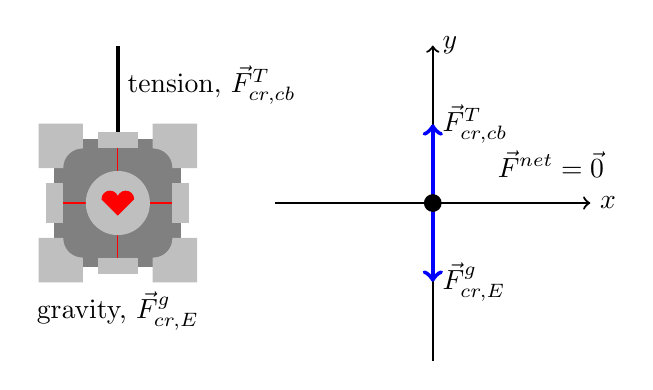
\begin{tikzpicture}
			\begin{scope}[shift={(-2,0)}]
				%\draw[thick] (-1,1) -- (1,1) -- (1,-1) -- (-1,-1) -- cycle;
				\filldraw[gray] (-0.8,0.8) -- (0.8,0.8) -- (0.8,-0.8) -- (-0.8,-0.8) -- cycle;
				\filldraw[lightgray] (-1,1) -- (-0.45,1) -- (-0.45,0.7) arc (90:180:0.25) -- (-1,0.45) -- cycle;
				\filldraw[lightgray,rotate=90] (-1,1) -- (-0.45,1) -- (-0.45,0.7) arc (90:180:0.25) -- (-1,0.45) -- cycle;
				\filldraw[lightgray,rotate=180] (-1,1) -- (-0.45,1) -- (-0.45,0.7) arc (90:180:0.25) -- (-1,0.45) -- cycle;
				\filldraw[lightgray,rotate=270] (-1,1) -- (-0.45,1) -- (-0.45,0.7) arc (90:180:0.25) -- (-1,0.45) -- cycle;
				\draw[red] (-0.8,0) -- (0.8,0);
				\draw[red] (0,-0.8) -- (0,0.8);
				\filldraw[lightgray] (-0.9,0.25) -- (-0.7,0.25) -- (-0.7,-0.25) -- (-0.9,-0.25) -- cycle;
				\filldraw[lightgray,rotate=90] (-0.9,0.25) -- (-0.7,0.25) -- (-0.7,-0.25) -- (-0.9,-0.25) -- cycle;
				\filldraw[lightgray,rotate=180] (-0.9,0.25) -- (-0.7,0.25) -- (-0.7,-0.25) -- (-0.9,-0.25) -- cycle;
				\filldraw[lightgray,rotate=270] (-0.9,0.25) -- (-0.7,0.25) -- (-0.7,-0.25) -- (-0.9,-0.25) -- cycle;
				\filldraw[lightgray] (0,0) circle (0.4);
				\filldraw[red] (-0.2,0.05) arc (180:0:0.1) arc (180:0:0.1) -- (0,-0.15) -- cycle;
				\draw[ultra thick] (0,0.9) -- (0,2);
				\node[anchor=north] at (0,-1) {gravity, $\vec{F}^{g}_{cr,E}$};
				\node[anchor=west] at (0,1.5) {tension, $\vec{F}^{T}_{cr,cb}$};
			\end{scope}
			\FBDaxes{2,0}{0}{axes}
			\FBDvectorXY{axes}{0,1}{FT}
			\node[anchor=west] at (FTtip) {$\vec{F}^{T}_{cr,cb}$};
			\FBDvectorXY{axes}{0,-1}{FG}
			\node[anchor=west] at (FGtip) {$\vec{F}^{g}_{cr,E}$};
			\FBDdot{axes}
			\node at ($(axes) + (1.5,0.5)$) {$\vec{F}^{net}=\vec{0}$};
		\end{tikzpicture}
	\end{figure}
}
\ProblemSub{\Brick}{
	(b) A brick is falling from the roof a three-story building.
}
\Solution{\BrickFig}{
	\begin{figure}[h]
		\centering
		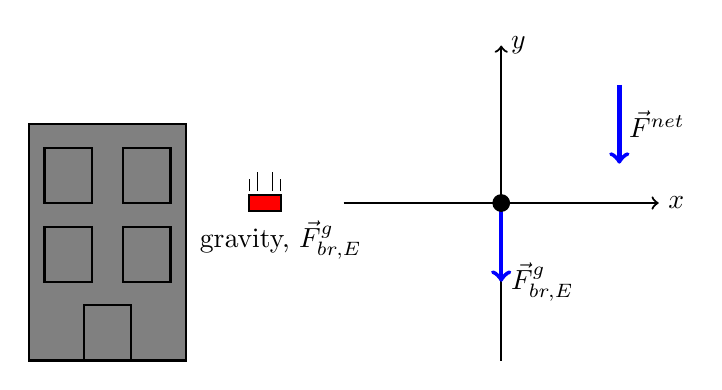
\begin{tikzpicture}
			\begin{scope}[shift={(-3,0)}]
				\filldraw[gray,draw=black,thick] (-1,-2) -- (1,-2) -- (1,1) -- (-1,1) -- cycle;
				\draw[thick] (-0.3,-2) -- (0.3,-2) -- (0.3,-1.3) -- (-0.3,-1.3) -- cycle;
				\draw[thick,shift={(0.5,1)}] (-0.3,-2) -- (0.3,-2) -- (0.3,-1.3) -- (-0.3,-1.3) -- cycle;
				\draw[thick,shift={(-0.5,1)}] (-0.3,-2) -- (0.3,-2) -- (0.3,-1.3) -- (-0.3,-1.3) -- cycle;
				\draw[thick,shift={(0.5,2)}] (-0.3,-2) -- (0.3,-2) -- (0.3,-1.3) -- (-0.3,-1.3) -- cycle;
				\draw[thick,shift={(-0.5,2)}] (-0.3,-2) -- (0.3,-2) -- (0.3,-1.3) -- (-0.3,-1.3) -- cycle;
			\end{scope}
			\filldraw[red,draw=black,thick,shift={(-1,0)}] (-0.2,-0.1) -- (0.2,-0.1) -- (0.2,0.1) -- (-0.2,0.1) -- cycle;
			\draw (-1.2,0.15) -- (-1.2,0.3);
			\draw (-0.8,0.15) -- (-0.8,0.3);
			\draw (-1.1,0.15) -- (-1.1,0.4);
			\draw (-0.9,0.15) -- (-0.9,0.4);
			\node[anchor=north] at (-0.8,-0.1) {gravity, $\vec{F}^{g}_{br,E}$};
			\FBDaxes{2,0}{0}{axes}
			\FBDvectorXY{axes}{0,-1}{FG}
			\node[anchor=west] at (FGtip) {$\vec{F}^{g}_{br,E}$};
			\FBDdot{axes}
			\FBDvectorXY{$(axes)+(1.5,1.5)$}{0,-1}{Fnet}
			\node[anchor=west] at ($(Fnettip) + (0,0.5)$) {$\vec{F}^{net}$};
		\end{tikzpicture}
	\end{figure}
}
\ProblemSub[34]{\PushBox}{
	(c) A girl is pushing a box across a rough horizontal floor at a steadily increasing speed.
}
\Solution{\PushBoxFig}{We will use the subscript $S$ (as in ``surface'') for the floor.
	
	\begin{figure}[h]
		\centering
		\begin{tikzpicture}
			\node at (-3.5,0) {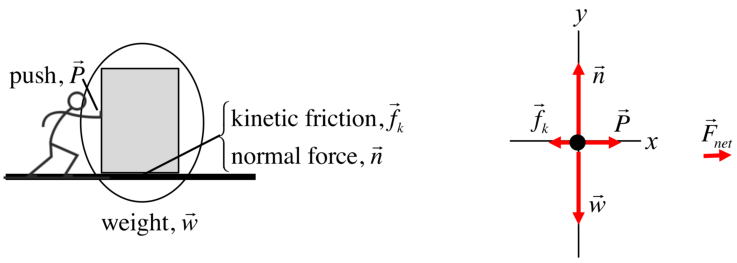
\includegraphics[trim={0 0 5cm 0},clip]{\FileDepth/Activities/Crate_Brick_Box_Car_FBDs/Girl_Pushing_the_Box_with_FBD}};
			\filldraw[white,shift={(-7.1,0.7)}] (0,0) rectangle (1.3,0.5);
			\node[anchor=south east] at (-5.7,0.7) {normal force, $\vec{F}^{N}_{BG}$};
			\filldraw[white,shift={(-5.6,-1.8)}] (0,0) rectangle (1.7,0.5);
			\node[anchor=south west] at (-5.6,-1.8) {gravity, $\vec{F}^{g}_{BE}$};
			\filldraw[white,shift={(-1,-0.6)}] (0,0) rectangle (0.5,0.5);
			\node[anchor=west] at (-1,-0.45) {$\vec{F}^{N}_{BS}$};
			\filldraw[white,shift={(-0.7,0)}] (0,0) rectangle (0.5,0.5);
			\node[anchor=west] at (-0.7,0.2) {$\vec{F}^{kf}_{BS}$};
			\FBDaxes{2.3,0}{0}{axes}
			\FBDvectorXY{axes}{0,-1.5}{FG}
			\node[anchor=west] at (FGtip) {$\vec{F}^{g}_{BE}$};
			\FBDvectorXY{axes}{0,1.5}{FNg}
			\node[anchor=west] at (FNgtip) {$\vec{F}^{N}_{BS}$};
			\FBDvectorXY{axes}{1,0}{FNp}
			\node[anchor=north] at (FNptip) {$\vec{F}^{N}_{BG}$};
			\FBDvectorXY{axes}{-0.5,0}{FK}
			\node[anchor=north] at (FKtip) {$\vec{F}^{kf}_{BS}$};
			\FBDvectorXY{$(axes)+(1.5,1)$}{0.5,0}{Fnet}
			\node[anchor=south] at (Fnettip) {$\vec{F}^{net}$};
			\FBDdot{axes}
		\end{tikzpicture}
	\end{figure}
}
\ProblemSub{\Brakes}{
	(d) You've slammed on your car brakes while going down a hill. The car is skidding to a stop.
}
\Solution{\BrakesFig}{
	\begin{figure}[h]
		\centering
		\begin{tikzpicture}
			\node at (-2.3,0) {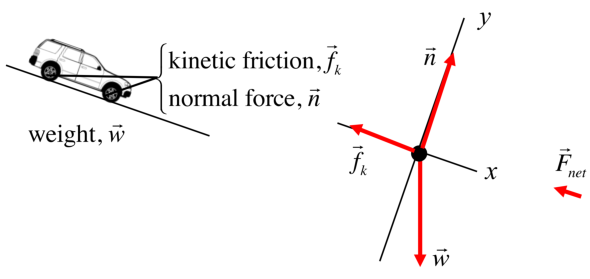
\includegraphics[trim={0 0 4.51cm 0},clip]{\FileDepth/Activities/Crate_Brick_Box_Car_FBDs/Car_Skidding_Downhill_with_FBD}};
			\filldraw[white,shift={(0.1,0.5)}] (0,0) rectangle (0.5,0.5);
			\node[anchor=west] at (0.4,1.3) {$\vec{F}^{kf}_{BS}$};
			\node[anchor=west] at (0.1,0.7) {$\vec{F}^{N}_{BS}$};
			\filldraw[white,shift={(-4.6,-0.2)}] (0,0) rectangle (1.7,0.5);
			\node[anchor=south west] at (-4.6,-0.2) {gravity, $\vec{F}^{g}_{BE}$};
			\FBDaxes{3,0}{-30}{axes}
			\FBDvectorMA{axes}{1.2}{150}{FK}
			\node[anchor=south] at (FKtip) {$\vec{F}^{kf}_{CS}$};
			\FBDvectorMA{axes}{1.5}{60}{FN}
			\node[anchor=west] at (FNtip) {$\vec{F}^{N}_{CS}$};
			\FBDvectorXY{axes}{0,-1.7}{FG}
			\node[anchor=north] at (FGtip) {$\vec{F}^{g}_{CE}$};
			\FBDvectorMA{$(axes)+(2,0)$}{0.4}{150}{Fnet}
			\node[anchor=south] at (Fnettip) {$\vec{F}^{net}$};
			\FBDdot{axes}
		\end{tikzpicture}
	\end{figure}
}
\Problem{Free Fall from FBD}{\Falling}{
	Using Newton's 2nd law, show that if air resistance is negligible the acceleration of a freely falling object equals the acceleration due to gravity. [Hint: see your free-body diagram from Activity 1(b).]
}
\Solution{\FallingSol}{Newton's 2nd law states that the net force (the sum of \textbf{all} forces on an object) is proportional to the acceleration of the object. In particular,
	\[
	\vec{F}_{net} = m\vec{a}.
	\]
	In the specific case of an object in free fall, the only (non-negligible) force on the object is the force of gravity, $ \vec{F}_{g} = m\vec{g} $. As such, $ \vec{F}_{net} = m\vec{g} $, and we can apply Newton's 2nd law to see
	\[
	\begin{split}
		\cancel{m}\vec{a} & = \cancel{m}\vec{g} \\
		\vec{a} & = \vec{g}.
	\end{split}
	\]
	As such, acceleration in free fall has no dependence upon the mass of the object. Though a more massive object weighs more (has a greater force of gravity upon it), it also has more inertia, and its velocity is therefore more resistant to change.
}
\Problem{Suitcase Pull}{\SuitcasePull}{
	Using a handle at the end of a 15 kg suitcase, a boy is pulling it to the right across a rough horizontal floor with a force of 55 N at an angle of 25$ ^{\circ} $ above the horizontal. The force of kinetic friction between the suitcase and the floor is 75 N. Neglect air resistance and assume that the suitcase doesn’t leave the floor.
}

\ProblemSub{\SuitcasePullA}{
	(a) Draw a sketch showing the suitcase and the boy.
}
\Solution{\SuitcasePullASol}{
	\begin{figure}[h]
		\centering
		
\includegraphics{\FileDepth/Activities/Suitcase_Pull/Boy_Pulling_Suitcase}
	\end{figure}
}
\ProblemSub{\SuitcasePullB}{
	(b) Identify the forces acting on the suitcase. For each force state whether it is a contact force or a long-range force.
}
\Solution{\SuitcasePullBSol}{The \textbf{force of gravity} is the only \textit{non-contact} force in this situation, pulling the suitcase toward the floor. To hold it up (at least partially), the floor exerts a \textbf{normal force} back on the suitcase, which is a \textit{contact} force. The floor also exerts a second \textit{contact} force on the suitcase: \textbf{kinetic friction}. The fourth and final force on the suitcase is \textbf{the boy's pull}, which is a \textit{contact} force. Since it is at an angle, some of it goes toward supporting the weight of the suitcase, which means the normal force does not have to be equal in magnitude to the force of gravity.
	
What type of force is the boy's pull? It depends on the choice of system. If the suitcase handle is not in the system with the suitcase, we might say we have a force of tension on the suitcase by the handle. In the more likely case that we include the handle in the system with the suitcase, then the boy's fingers are pushing on the inner surface of the handle, which would be a normal force. This is the choice I will make on the free body diagram.
}
\ProblemSub{\SuitcasePullC}{
	(c) Draw a free-body diagram for the suitcase. Use the particle model.
}
\Solution{\SuitcasePullCSol}{I will use the subscript $S$ (for ``surface'') to denote the floor, and $sc$ to denote the suitcase.
	
	Since the boy's pull exerts only 55 N at an angle of 25$ ^{\circ} $ above the horizontal, it will be overwhelmed by the oppositely oriented force of kinetic friction, which exerts 75 N horizontally on the suitcase:
	\[
	75 \text{ N} > (55\text{ N})\cos(25^{\circ}).
	\]
	Thus, the net force is to the left, and the suitcase is slowing down.
	\begin{figure}[h]
		\centering
		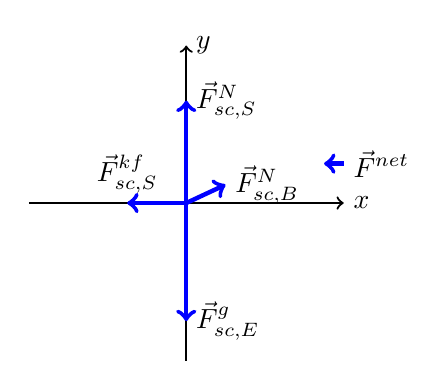
\begin{tikzpicture}
			\FBDaxes{0,0}{0}{axes}
			\FBDvectorMA{axes}{0.55}{25}{P}
			\node[anchor=west] at (Ptip) {$\vec{F}^{N}_{sc,B}$};
			\FBDvectorXY{axes}{-0.75,0}{FK}
			\node[anchor=south] at (FKtip) {$\vec{F}^{kf}_{sc,S}$};
			\FBDvectorXY{axes}{0,-1.5}{FG}
			\node[anchor=west] at (FGtip) {$\vec{F}^{g}_{sc,E}$};
			\FBDvectorXY{axes}{0,1.3}{FN}
			\node[anchor=west] at (FNtip) {$\vec{F}^{N}_{sc,S}$};
			\FBDvectorXY{2,0.5}{-0.25,0}{Fnet}
			\node[anchor=west] at (2,0.5) {$\vec{F}^{net}$};
		\end{tikzpicture}
	\end{figure}
}
\end{document}